%---------------------------------------------------------------------
%
%                          Cap�tulo 4
%
%---------------------------------------------------------------------

\chapter{Arquitectura del generador de historias}

\begin{FraseCelebre}
\begin{Frase}
	Comentar el c�digo es como limpiar el cuarto de ba�o; nadie quiere hacerlo, pero el resultado es siempre una experiencia m�s agradable para uno mismo y sus invitados
\end{Frase}
\begin{Fuente}
	Ryan Campbell
\end{Fuente}
\end{FraseCelebre}

Al momento de empezar a crear una historia podemos plantearnos diferentes enfoques con el fin de abordar esta cuesti�n de la manera mas sencilla posible. Para nosotros, el aspecto mas importante de esto son los personajes. Queremos hacer historias que se centren en estos ya que ser�n estos quienes al momento de interactuar entre si, generar�n la historia que deseemos.

Para hacer que existan los personajes dentro del sistema es necesario definirlos y darles las herramientas necesarias para que estos puedan interactuar. Dicho esto, los personajes deben existir dentro del sistema multi-agente.

El SMA es el componente capaz de dotar a los personajes de las herramientas que les permiten enviar mensajes para comunicarse con otros personajes y existir como agentes software. Usando JADE, este sistema nos permite controlar la existencia de los agentes y poder manipularlos como tal.

El siguiente enfoque tiene mas que ver con el aspecto del entorno de la historia. Tener varios personajes en la historia no implica nada si estos no disponen de un entorno sobre el cual desarrollar sus acciones y vivencias. Es necesario ahora otorgar al sistema un poco m�s de profundidad en el asunto, necesitamos a�adir el mundo.

El Mundo, o agente Mundo, es un componente que permitir� a los personajes disponer de un nuevo espacio, un lugar donde queden reflejadas sus acciones. Sin la existencia del Mundo podr�amos decir que los personajes viven en la nada, visto de otra forma, es como si todos estuviesen en una habitaci�n vac�a, un espacio unidimensional en el cual no tendr�a sentido realizar acciones como moverse, negociar con terceros personajes, dudar...

La existencia del Mundo como nueva dimensi�n espacial aporta a los personajes la capacidad de existir en un plano. Los personajes dejan de conocer la situaci�n de otros y llegan a la necesidad de interactuar con su entorno para poder realizar acciones relevantes en una historia.

Ahora que ya tenemos un ecosistema creado con los personajes y su entorno, necesitamos de un sistema capaz de otorgar la l�gica o inteligencia a los personajes. Dicho sistema es el planificador. El planificador es el componente que permite a los personajes "pensar" en la secuencia de acciones que deben realizar para poder cumplir sus objetivos dentro de la historia. Estas acciones ayudar�n al personaje desde decidir a cual direcci�n moverse hasta en que momento pelear con otro personaje.

Con todo esto tenemos descrito el n�cleo importante de nuestro sistema. Se han juntado los componentes m�nimos para poder generar una historia. A�n as�, todav�a el usuario no est� incluido dentro de todo esto, y no tiene sentido tener un sistema que trabaje para s� en lugar de dejarle a un usuario una copia de los resultados obtenidos.

Es necesario el uso de alg�n componente � sistema que nos permita recoger el flujo de historia final. Saber cu�les han sido los mensajes que intercambiaron los personajes y las acciones que realizaron. Usar un \textit{logger} nos permite guardar un registro del momento en el que ocurre cada eventos de la historia.

Sin embargo, al ser un sistema pensado para ser utilizado por un usuario, falta disponer de una capa que permita a este interactuar con el sistema. La interfaz gr�fica otorga al usuario la capacidad de visualizar informaci�n adicional durante el momento de la simulaci�n. Es mediante esta capa, que el usuario puede tambi�n a�adir nuevos elementos a la generaci�n de historias.

A continuaci�n hablaremos con m�s detalle sobre cada uno de estos componentes y sobre otras partes del sistema necesarias � que se ven afectadas por estos.

\newpage
%-------------------------------------------------------------------
\section{Diagrama de la arquitectura}

Para tener una referencia que nos permita visualizar de manera sencilla la arquitectura del proyecto, podemos fijarnos en la figura \ref{fig:ArquitecturaProyecto}.

\begin{figure}[h]
	\centering
	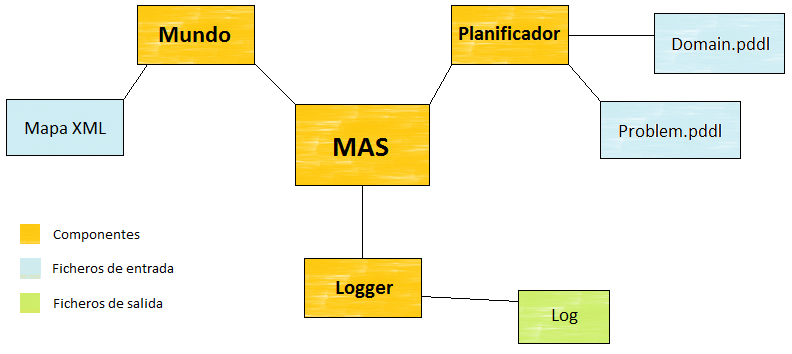
\includegraphics[width=0.8\textwidth]{Imagenes/arquitectura}
	\caption{Arquitectura del proyecto}
	\label{fig:ArquitecturaProyecto}
\end{figure}

%-------------------------------------------------------------------
\section{El Agente Mundo}
\label{cap4:sec:AgenteMundo}

%-------------------------------------------------------------------
\section{El Planificador}
\label{cap4:sec:Planificador}

%-------------------------------------------------------------------
\section{Sistemas Cargadores de Datos o SCD's}
\label{cap4:sec:Loaders}

%-------------------------------------------------------------------
\section{Interfaz Personaje}
\label{cap4:sec:InterfazPersonajes}

\section{Archivos de Configuraci�n}
